\chapter{計算実験}\label{computational_result}
\section{計算環境}
実験に用いるプログラムはPythonを用いて実装し, 計算機はMacBookAir2020 (CPU: 8 コア Apple M1 chip, メモリ: 8 GB LPDDR4)を用いて行った. 

\section{第一段階の求解結果}
整数計画ソルバー (Gurobi Optimizer ver. 9.5)を用いて計算した結果, 全ての問題例で最適解が得られた. 
出力の例を図\ref{first-no-rei}に示す. 
長方形内の番号はグループの番号を表す. 
灰色の長方形は, ランプを表す. \\

\begin{figure}[b]
    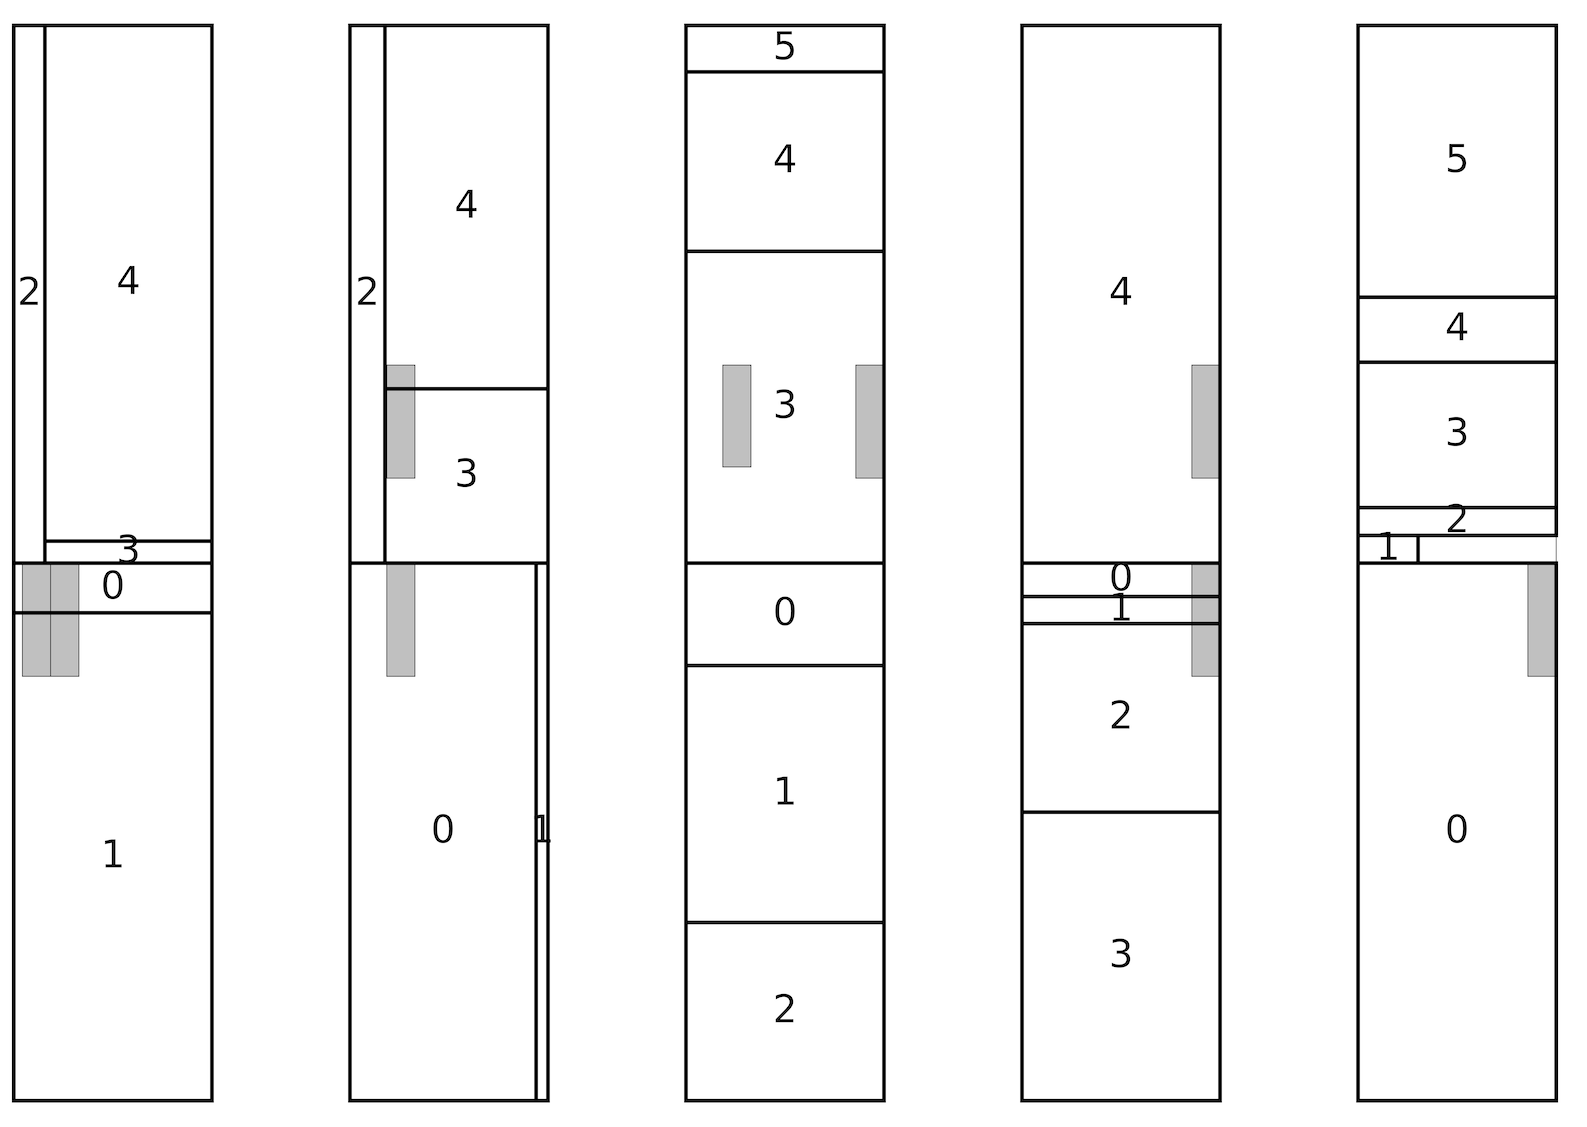
\includegraphics[scale=0.3, bb = 0 0 1 1]{5-first-no-rei.png}
    \caption{第一段階の出力の例}
    \label{first-no-rei}
\end{figure}
\clearpage


\section{第二段階の求解結果}
BL法による計算結果と, 出力される配置図の例を図\ref{second-no-rei}に示す. 
NF法による計算結果と, 出力される配置図の例を図\ref{nf-norei}に示す. 
配置図上の各長方形が車を表し, 色は揚げ地の種類を表す. \\

\begin{table}[h]
    % \tabcolsep = 10pt
        \centering
        \caption{近傍操作による解の改善}
        \label{review-local}
        \begin{tabular}{cccccccc}
        \hline
        & & \multicolumn{3}{c}{初期解 (BL法)} & \multicolumn{3}{c}{BL法 $+$ 局所探索} \\
        \hline
        問題番号 & 車の台数  & 余り (台)  & 充填率 (\%) & 計算時間 (s) & 余り (台)  & 充填率 (s)  & 計算時間 (s)  \\
        \hline
        1    & 773  & 20      & 75.7     & 75.9     & 0       &  77.7    & 275.8     \\
        2    & 691  & 5       & 78.0     & 80.4     & 5       &  78.0    & 241.1     \\
        3    & 585  & 27      & 73.7     & 111.1    & 27      &  73.7    & 322.0     \\
        4    & 604  & 95      & 67.9     & 149.5    & 39      &  74.9    & 937.5     \\
        5    & 594  & 36      & 74.7     & 159.3    & 27      &  76.0    & 747.3     \\
        6    & 481  & 22      & 67.6     & 149.4    & 10      &  69.5    & 601.9     \\
        7    & 370  & 9       & 54.0     & 99.2     & 9       &  54.0    & 285.9     \\
        8    & 530  & 9       & 77.8     & 139.8    & 9       &  77.8    & 422.7     \\
        9    & 545  & 93      & 66.3     & 143.4    & 42      &  74.5    & 688.2     \\
        10   & 581  & 96      & 65.9     & 161.9    & 87      &  67.0    & 548.9     \\
        11   & 530  & 0       & 75.5     & 192.3    & 0       &  75.5    & 385.6     \\
        12   & 641  & 29      & 75.1     & 184.3    & 29      &  75.1    & 550.9     \\
        13   & 609  & 88      & 65.5     & 92.4     & 88      &  65.5    & 277.4     \\
        14   & 675  & 72      & 67.6     & 185.5    & 72      &  67.6    & 524.1     \\
        15   & 629  & 2       & 80.0     & 166.5    & 1       &  80.2    & 517.3     \\
        \hline
        \end{tabular}
\end{table}


\begin{table}[b]
    \centering
    \caption{近傍操作による解の改善 (NF法)}
    \label{review-local-nf}
    \begin{tabular}{cccccccc}
    \hline
        & & \multicolumn{3}{c}{初期解 (NF法)} & \multicolumn{3}{c}{NF法 $+$ 局所探索} \\
    \hline
    問題番号 & 車の台数  & 余り (台)  & 充填率 (\%) & 計算時間 (s) & 余り (台)  & 充填率 (s)  & 計算時間 (s)  \\
    \hline
    1    & 773  & 62      & 71.5     &  5.7     & 54      & 72.3     & 22.5       \\
    2    & 691  & 64      & 72.5     &  1.4     & 64      & 72.5     & 4.0      \\
    3    & 585  & 48      & 70.9     &  5.4     & 43      & 71.5     & 21.6       \\
    4    & 604  & 133     & 63.0     &  0.6     & 79      & 69.5     & 7.2      \\
    5    & 594  & 75      & 69.5     &  11.0    & 72      & 69.9     & 40.4       \\
    6    & 481  & 26      & 67.1     & 0.7      & 26      & 67.1     & 2.3          \\
    7    & 370  & 25      & 51.9     & 0.5      & 25      & 51.9     & 1.5       \\
    8    & 530  & 23      & 75.7     & 0.5      & 23      & 75.7     & 1.5       \\
    9    & 545  & 106     & 64.6     & 0.7      & 106     & 64.4     & 2.2        \\
    10   & 581  & 115     & 63.3     & 6.0      & 115     & 63.3     & 18.2       \\
    11   & 530  & 19      & 72.8     & 0.7      & 18      & 74.4     & 3.5      \\
    12   & 641  & 74      & 70.0     & 0.9      & 74      & 70.0     & 2.9       \\
    13   & 609  & 112     & 62.4     & 2.7      & 110     & 62.7     & 11.0       \\
    14   & 675  & 104     & 63.7     & 4.9      & 104     & 63.7     & 14.8      \\
    15   & 629  & 39      & 75.3     & 1.3      & 39      & 75.3     & 4.0      \\
    \hline
    \end{tabular}
\end{table}


\begin{figure}[p]
    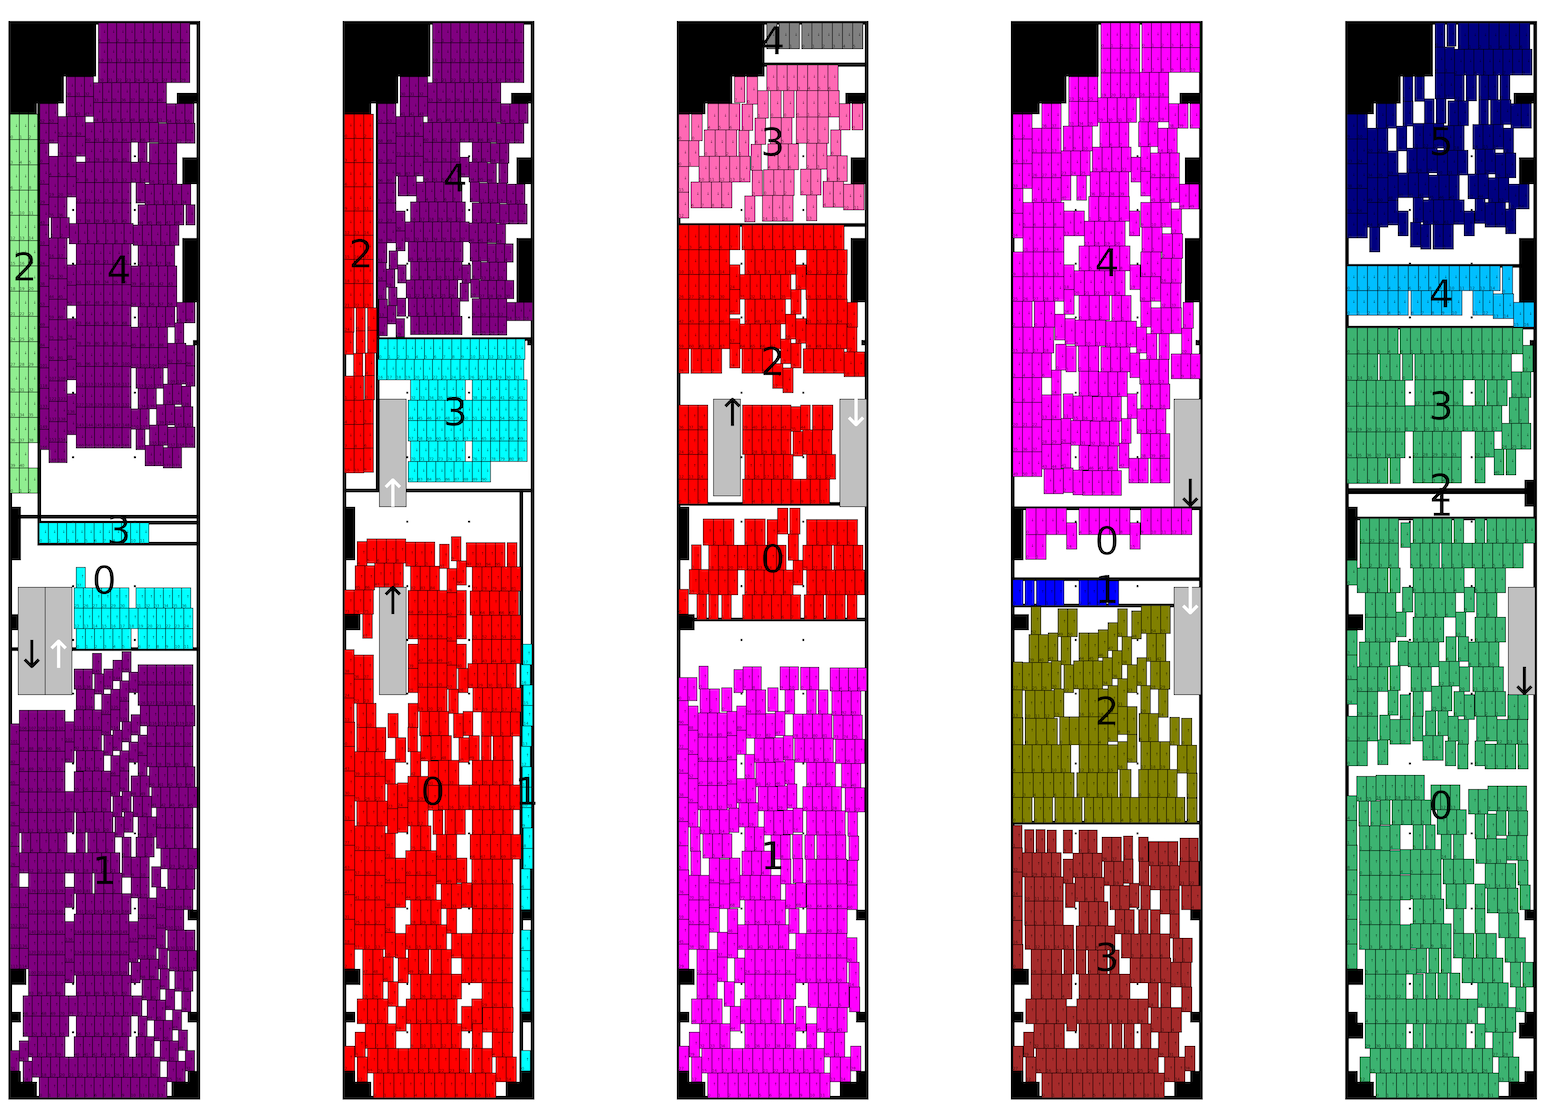
\includegraphics[scale=0.3, bb = 0 0 1 1]{5-second-no-rei.png}
    \caption{BL法による出力図の例}
    \label{second-no-rei}
\end{figure}

\begin{figure}[p]
    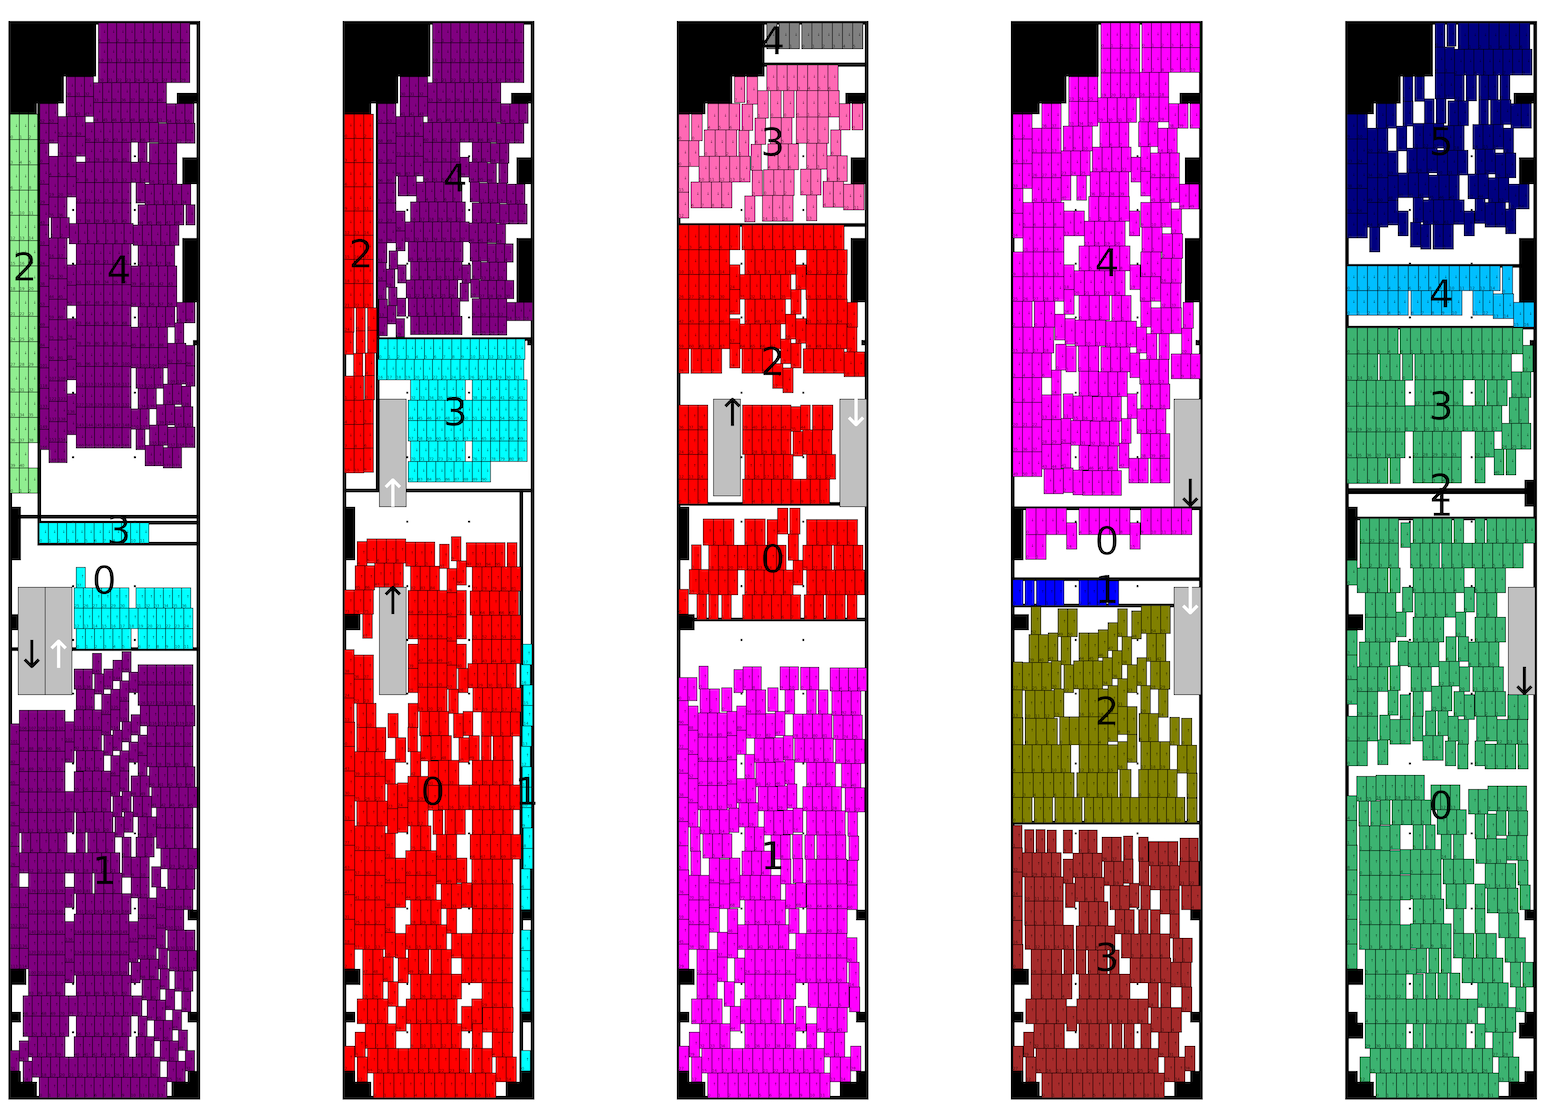
\includegraphics[scale=0.3, bb = 0 0 1 1]{5-second-no-rei.png}
    \caption{NF法による出力図の例}
    \label{nf-norei}
\end{figure}

